\documentclass[]{article}
\usepackage{lmodern}
\usepackage{amssymb,amsmath}
\usepackage{ifxetex,ifluatex}
\usepackage{fixltx2e} % provides \textsubscript
\ifnum 0\ifxetex 1\fi\ifluatex 1\fi=0 % if pdftex
  \usepackage[T1]{fontenc}
  \usepackage[utf8]{inputenc}
\else % if luatex or xelatex
  \ifxetex
    \usepackage{mathspec}
    \usepackage{xltxtra,xunicode}
  \else
    \usepackage{fontspec}
  \fi
  \defaultfontfeatures{Mapping=tex-text,Scale=MatchLowercase}
  \newcommand{\euro}{€}
\fi
% use upquote if available, for straight quotes in verbatim environments
\IfFileExists{upquote.sty}{\usepackage{upquote}}{}
% use microtype if available
\IfFileExists{microtype.sty}{%
\usepackage{microtype}
\UseMicrotypeSet[protrusion]{basicmath} % disable protrusion for tt fonts
}{}
\ifxetex
  \usepackage[setpagesize=false, % page size defined by xetex
              unicode=false, % unicode breaks when used with xetex
              xetex]{hyperref}
\else
  \usepackage[unicode=true]{hyperref}
\fi
\hypersetup{breaklinks=true,
            bookmarks=true,
            pdfauthor={},
            pdftitle={},
            colorlinks=true,
            citecolor=blue,
            urlcolor=blue,
            linkcolor=magenta,
            pdfborder={0 0 0}}
\urlstyle{same}  % don't use monospace font for urls
\usepackage{color}
\usepackage{fancyvrb}
\newcommand{\VerbBar}{|}
\newcommand{\VERB}{\Verb[commandchars=\\\{\}]}
\DefineVerbatimEnvironment{Highlighting}{Verbatim}{commandchars=\\\{\}}
% Add ',fontsize=\small' for more characters per line
\newenvironment{Shaded}{}{}
\newcommand{\KeywordTok}[1]{\textcolor[rgb]{0.00,0.44,0.13}{\textbf{{#1}}}}
\newcommand{\DataTypeTok}[1]{\textcolor[rgb]{0.56,0.13,0.00}{{#1}}}
\newcommand{\DecValTok}[1]{\textcolor[rgb]{0.25,0.63,0.44}{{#1}}}
\newcommand{\BaseNTok}[1]{\textcolor[rgb]{0.25,0.63,0.44}{{#1}}}
\newcommand{\FloatTok}[1]{\textcolor[rgb]{0.25,0.63,0.44}{{#1}}}
\newcommand{\ConstantTok}[1]{\textcolor[rgb]{0.53,0.00,0.00}{{#1}}}
\newcommand{\CharTok}[1]{\textcolor[rgb]{0.25,0.44,0.63}{{#1}}}
\newcommand{\SpecialCharTok}[1]{\textcolor[rgb]{0.25,0.44,0.63}{{#1}}}
\newcommand{\StringTok}[1]{\textcolor[rgb]{0.25,0.44,0.63}{{#1}}}
\newcommand{\VerbatimStringTok}[1]{\textcolor[rgb]{0.25,0.44,0.63}{{#1}}}
\newcommand{\SpecialStringTok}[1]{\textcolor[rgb]{0.73,0.40,0.53}{{#1}}}
\newcommand{\ImportTok}[1]{{#1}}
\newcommand{\CommentTok}[1]{\textcolor[rgb]{0.38,0.63,0.69}{\textit{{#1}}}}
\newcommand{\DocumentationTok}[1]{\textcolor[rgb]{0.73,0.13,0.13}{\textit{{#1}}}}
\newcommand{\AnnotationTok}[1]{\textcolor[rgb]{0.38,0.63,0.69}{\textbf{\textit{{#1}}}}}
\newcommand{\CommentVarTok}[1]{\textcolor[rgb]{0.38,0.63,0.69}{\textbf{\textit{{#1}}}}}
\newcommand{\OtherTok}[1]{\textcolor[rgb]{0.00,0.44,0.13}{{#1}}}
\newcommand{\FunctionTok}[1]{\textcolor[rgb]{0.02,0.16,0.49}{{#1}}}
\newcommand{\VariableTok}[1]{\textcolor[rgb]{0.10,0.09,0.49}{{#1}}}
\newcommand{\ControlFlowTok}[1]{\textcolor[rgb]{0.00,0.44,0.13}{\textbf{{#1}}}}
\newcommand{\OperatorTok}[1]{\textcolor[rgb]{0.40,0.40,0.40}{{#1}}}
\newcommand{\BuiltInTok}[1]{{#1}}
\newcommand{\ExtensionTok}[1]{{#1}}
\newcommand{\PreprocessorTok}[1]{\textcolor[rgb]{0.74,0.48,0.00}{{#1}}}
\newcommand{\AttributeTok}[1]{\textcolor[rgb]{0.49,0.56,0.16}{{#1}}}
\newcommand{\RegionMarkerTok}[1]{{#1}}
\newcommand{\InformationTok}[1]{\textcolor[rgb]{0.38,0.63,0.69}{\textbf{\textit{{#1}}}}}
\newcommand{\WarningTok}[1]{\textcolor[rgb]{0.38,0.63,0.69}{\textbf{\textit{{#1}}}}}
\newcommand{\AlertTok}[1]{\textcolor[rgb]{1.00,0.00,0.00}{\textbf{{#1}}}}
\newcommand{\ErrorTok}[1]{\textcolor[rgb]{1.00,0.00,0.00}{\textbf{{#1}}}}
\newcommand{\NormalTok}[1]{{#1}}
\usepackage{graphicx,grffile}
\makeatletter
\def\maxwidth{\ifdim\Gin@nat@width>\linewidth\linewidth\else\Gin@nat@width\fi}
\def\maxheight{\ifdim\Gin@nat@height>\textheight\textheight\else\Gin@nat@height\fi}
\makeatother
% Scale images if necessary, so that they will not overflow the page
% margins by default, and it is still possible to overwrite the defaults
% using explicit options in \includegraphics[width, height, ...]{}
\setkeys{Gin}{width=\maxwidth,height=\maxheight,keepaspectratio}
\setlength{\parindent}{0pt}
\setlength{\parskip}{6pt plus 2pt minus 1pt}
\setlength{\emergencystretch}{3em}  % prevent overfull lines
\providecommand{\tightlist}{%
  \setlength{\itemsep}{0pt}\setlength{\parskip}{0pt}}
\setcounter{secnumdepth}{0}

\date{}

% Redefines (sub)paragraphs to behave more like sections
\ifx\paragraph\undefined\else
\let\oldparagraph\paragraph
\renewcommand{\paragraph}[1]{\oldparagraph{#1}\mbox{}}
\fi
\ifx\subparagraph\undefined\else
\let\oldsubparagraph\subparagraph
\renewcommand{\subparagraph}[1]{\oldsubparagraph{#1}\mbox{}}
\fi

\begin{document}
	\title{\huge\textbf{Distance Transform}\LARGE \\Project: Marker-based Localization}
	\author{Niharika Jayanthi, Dheeraj Kamath \\Mentor: Sanam Shakya}
	\maketitle
	\pagebreak
\section{Goal}\label{goal}

\begin{itemize}
\tightlist
\item
  To understand what is distance transformation.
\item
  Learn about chessboard, Euclidean and city-blocks distance metrics.
\item
  Learn how to code for distance transformation in python.
\end{itemize}

\section{Theory}\label{theory}

\subsection{Working Principle}\label{working-principle}

\subsubsection{Introduction}\label{introduction}

Distance transform is an operator that transforms the values of pixels
in an image according to their distance from the boundary of the object.
The farther a pixel is from the image boundary, the higher a value it
gets. This would result in a transformed image where the area near and
within the boundary will be dark whereas the area near the center of the
image will be white. \\

To put it in different words, a pixel in an image can have a value equal
to the number of erosions required to be performed to make it disappear. \\

Distance transform operations can be classified into several types,
depending upon the way the distance of a pixel from the boundary has
been calculated (Distance metrics). Below are the three common distance
metrics- \\

\begin{itemize}
\tightlist
\item
  \textbf{Chessboard Distance}
\end{itemize}

This is analogous to a King on the chessboard, which can move
horizontally, vertically and diagonally. All moves are considered equal
to each other. Hence, distance between two points (x1, y1) and (x2, y2)
is calculated as-

\begin{verbatim}
D = max(|x2 - x1|,|y2 - y1|)
\end{verbatim}
~\\ \\ \\ \\ \\ \\ \\ \\ \\ \\  
\begin{figure}[htbp]
\begin{center}
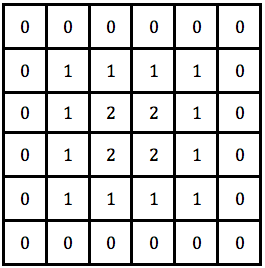
\includegraphics[width = 7cm]{images/Distance Transform/Images/Chessboard Distance.png}
\caption{Chessboard Distance}
\end{center}
\end{figure}

In the above image, each cell represents a pixel. As you can see, the
value of the pixel increases as it moves away from the boundary. This
distance is also known as Chebyshev distance. \\

\begin{itemize}
\tightlist
\item
  \textbf{Euclidean Distance}
\end{itemize}

This is equal to the length of the line segment formed by joining two
points. The following formula is used to calculate Euclidean distance
between two points A(x1, y1) and B(x2, y2)-

\begin{verbatim}
D = squareRoot( (x2 - x1)^2 + (y2 - y1)^2 )
\end{verbatim}
~\\ \\ \\ \\ \\
\begin{figure}[htbp]
\begin{center}
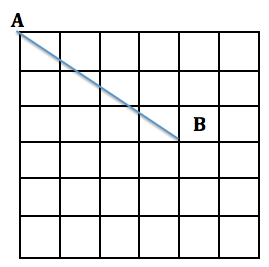
\includegraphics[width = 7cm]{images/Distance Transform/Images/Euclidean Distance.png}
\caption{Euclidean Distance}
\end{center}
\end{figure}

It is evident from the above example that the direct, straight distance
between the two points is calculated.

\begin{itemize}
\tightlist
\item
  \textbf{City-blocks Distance}
\end{itemize}

Also known as Taxicab distance or Manhattan distance, this method
measures distance by traveling along grid lines. Therefore, diagonal
moves are not possible. The formula for distance between two points
A(x1, y1) and B(x2, y2) is-

\begin{verbatim}
D = |x2 - x1| + |y2 - y1|
\end{verbatim}

\begin{figure}[htbp]
\centering
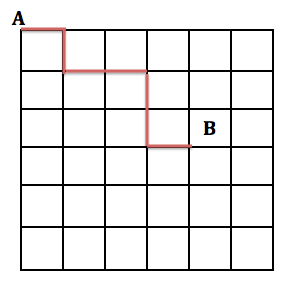
\includegraphics[width = 7cm]{images/Distance Transform/Images/City blocks Distance.png}
\caption{City Blocks distance}
\end{figure}
~\\ \\ \\ \\ \\ \\ \\ \\ \\ \\ \\ \\
In the above example, you can see how path can either move horizontally
or vertically only. The total distance would therefore be the sum of the
differences in x and y coordinates respectively.

\subsection{Applications}\label{applications}

\begin{itemize}
\tightlist
\item
  It is used to generate skeletons of images. Skeletons depict the
  connectivity, length and width of an image.
\item
  Distance transform can be applied in robotics for navigation and
  pathfinding.
\item
  Font smoothing and rendering also use distance transform.
\item
  3D modelling uses signed distance fields.
\end{itemize}

\subsection{Example}\label{example}

Consider the following image with different shapes- \\ \\

\begin{figure}[htbp]
\begin{center}
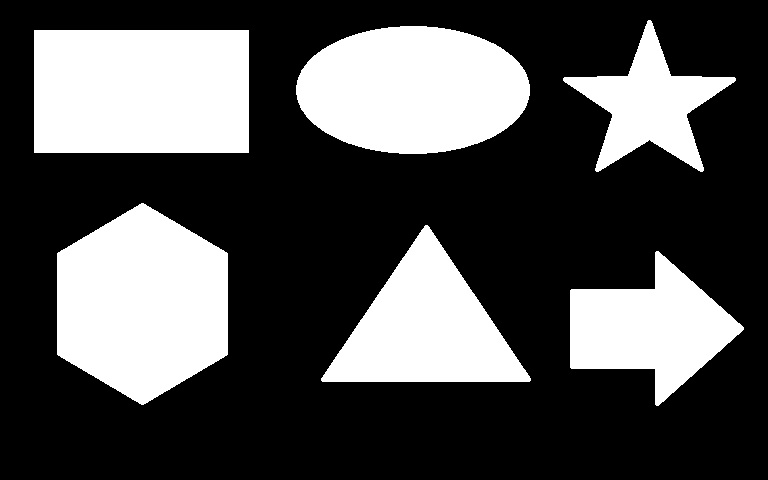
\includegraphics[width = 7cm]{images/Distance Transform/Images/example.jpg}
\caption{EXAMPLE}
\end{center}
\end{figure}
~\\ \\ \\ \\ \\ \\ \\
On performing distance transformation, it will look like this-

\begin{figure}[htbp]
\begin{center}
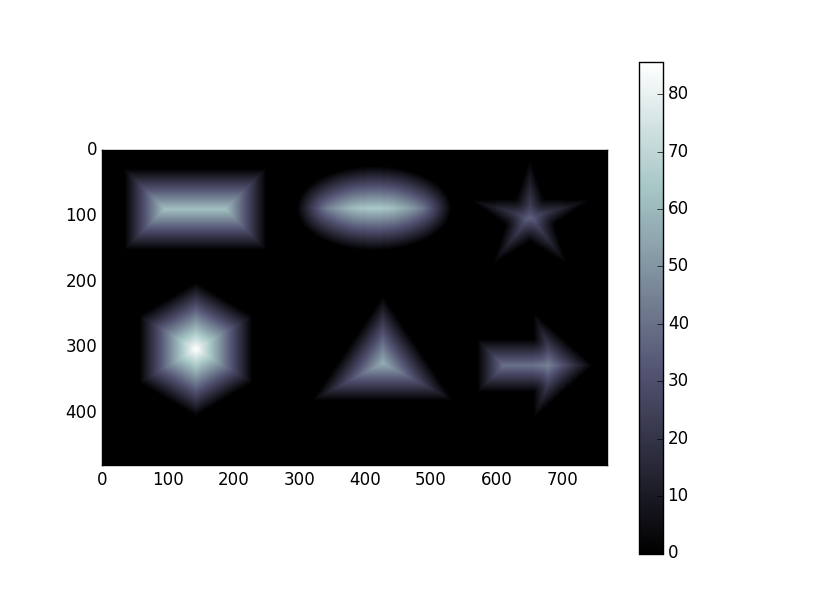
\includegraphics[width = 10cm]{images/Distance Transform/Images/Result.png}
\caption{Result}
\end{center}
\end{figure}
~\\ \\ \\
\section{Code}\label{code}

The main function used for distance transformation is-

\begin{Shaded}
\begin{Highlighting}[]
\NormalTok{cv2.distanceTransform(src, distanceType, maskSize)}
\end{Highlighting}
\end{Shaded}

Here,

\begin{verbatim}
src:          8-bit binary source image
distanceType: Type of distance. It can be CV_DIST_L1, CV_DIST_L2 or CV_DIST_C
maskSize:     Size of distance transform mask
\end{verbatim}
~\\ \\
\subsection{Explaining the code}\label{explaining-the-code}

\begin{itemize}
\tightlist
\item
  Let us first import the required packages.
\end{itemize}

\begin{Shaded}
\begin{Highlighting}[]
    \ImportTok{import} \NormalTok{cv2}
    \ImportTok{import} \NormalTok{matplotlib.pyplot }\ImportTok{as} \NormalTok{plt}
\end{Highlighting}
\end{Shaded}

cv2 package is required as it contains the distance transform function.
Matplotlib is needed to plot our images on the window.

\begin{itemize}
\tightlist
\item
  Next, we must read the image and convert it to a grayscale image.
\end{itemize}

\begin{Shaded}
\begin{Highlighting}[]
    \NormalTok{img }\OperatorTok{=} \NormalTok{cv2.imread(}\StringTok{'example.jpg'}\NormalTok{)}
    \NormalTok{gray }\OperatorTok{=} \NormalTok{cv2.cvtColor(img, cv2.COLOR_BGR2GRAY)}
\end{Highlighting}
\end{Shaded}

\begin{itemize}
\tightlist
\item
  We need a binary image as input for distance transform. So gray will
  be converted into a binary image using thresholding.
\end{itemize}

\begin{Shaded}
\begin{Highlighting}[]
    \NormalTok{ret, th }\OperatorTok{=} \NormalTok{cv2.threshold(gray, }\DecValTok{127}\NormalTok{, }\DecValTok{255}\NormalTok{, cv2.THRESH_BINARY)}
\end{Highlighting}
\end{Shaded}

\begin{itemize}
\tightlist
\item
  We can now perform distance transformation on th.
\end{itemize}

\begin{Shaded}
\begin{Highlighting}[]
    \NormalTok{distance }\OperatorTok{=} \NormalTok{cv2.distanceTransform(th, cv2.cv.CV_DIST_L2, }\DecValTok{5}\NormalTok{)}
\end{Highlighting}
\end{Shaded}

\begin{itemize}
\tightlist
\item
  Now, let us display the grayscale and distance transformed image on a
  window. First, we create a new window.
\end{itemize}

\begin{Shaded}
\begin{Highlighting}[]
    \NormalTok{plt.figure(}\DecValTok{0}\NormalTok{)}
\end{Highlighting}
\end{Shaded}

\begin{itemize}
\tightlist
\item
  The grayscale image will be plotted on the left side of the window
  with the following code-
\end{itemize}

\begin{Shaded}
\begin{Highlighting}[]
    \NormalTok{plt.subplot(}\DecValTok{121}\NormalTok{)}
    \NormalTok{plot }\OperatorTok{=} \NormalTok{plt.imshow(gray)}
    \NormalTok{plot.set_cmap(}\StringTok{'bone'}\NormalTok{)}
\end{Highlighting}
\end{Shaded}

By plt.subplot(121), we create a 1 row by 2 columns grid and position
the subplot in the first subplot.

\begin{itemize}
\tightlist
\item
  Now, we plot the second image on the right side of the window.
\end{itemize}

\begin{Shaded}
\begin{Highlighting}[]
    \NormalTok{plt.subplot(}\DecValTok{122}\NormalTok{)}
    \NormalTok{plot }\OperatorTok{=} \NormalTok{plt.imshow(distance)}
    \NormalTok{plot.set_cmap(}\StringTok{'bone'}\NormalTok{)}
\end{Highlighting}
\end{Shaded}

\begin{itemize}
\tightlist
\item
  Finally, we display our window using-
\end{itemize}

\begin{Shaded}
\begin{Highlighting}[]
    \NormalTok{plt.show()}
\end{Highlighting}
\end{Shaded}

\section{References}\label{references}

\begin{itemize}
\tightlist
\item
  http://homepages.inf.ed.ac.uk/rbf/HIPR2/distance.htm
\item
  http://homepages.inf.ed.ac.uk/rbf/HIPR2/metric.htm
\item
  http://en.wikipedia.org/wiki/Distance\_transform
\item
  http://docs.opencv.org/modules/imgproc/doc/miscellaneous\_transformations.html\#distancetransform
\item
  http://matplotlib.org/api/pyplot\_api.html
\end{itemize}



\end{document}
